\section{Bianchi Type~I Geometry}\label{sec:geometry}
%======================================================================

\subsection{The Wainwright--Hsu Variables}

In the orthonormal-frame approach of Wainwright and Hsu \cite{WainwrightEllis1997}, the LRS (locally rotationally symmetric) Bianchi Type~I spacetime has the metric
\begin{equation}
\dd s^2 = -\dd t^2 + a_1(t)^2\,\dd x^2 + a_2(t)^2\,\dd y^2 + a_3(t)^2\,\dd z^2\,,
\end{equation}
where the mean scale factor is $a = (a_1 a_2 a_3)^{1/3}$ and the mean Hubble rate is $H = \dot{a}/a$.  The shear tensor $\sigma_{ij}$ measures the anisotropic part of the expansion:
\begin{equation}
\sigma_{ij} = \frac{1}{2}(\dot{h}_{ij} - \frac{2}{3}\theta\,h_{ij})\,,
\end{equation}
where $h_{ij}$ is the spatial metric and $\theta = 3H$ is the volume expansion scalar.

The Hubble-normalised shear variables are
\begin{equation}
\Sigma_\pm = \frac{\sigma_\pm}{H}\,,
\end{equation}
with the total shear parameter $\Sigma^2 = \Sigma_+^2 + \Sigma_-^2$.  For LRS symmetry ($\Sigma_- = 0$), the evolution equation is
\begin{equation}
\frac{d\Sigma_+}{dN} = -(2-q)\,\Sigma_+ + \Pi_+\,,\label{eq:dSp}
\end{equation}
where $N = \ln a$ is the e-fold time, $q$ is the deceleration parameter, and $\Pi_+$ is the Hubble-normalised anisotropic stress from free-streaming neutrinos.

For a radiation-dominated universe with equation of state $w = 1/3$, the deceleration parameter is
\begin{equation}
q = 1 + \Sigma^2\,.
\end{equation}
In the FLRW limit ($\Sigma = 0$), $q = 1$ and we recover standard radiation-dominated deceleration.

\subsection{The Friedmann Constraint}

The Friedmann equation in Hubble-normalised form is
\begin{equation}
\Omega = 1 - \Sigma_+^2 - \Sigma_-^2\,,\label{eq:friedmann}
\end{equation}
where $\Omega = \rho/(3H^2)$ is the density parameter.  This is enforced algebraically at each timestep, not as a differential equation.  The physical Hubble rate is then
\begin{equation}
\boxed{H = \frac{H_\FLRW}{\sqrt{1 - \Sigma^2}}\,,}\label{eq:hubble}
\end{equation}
which is enhanced by shear.  For small $\Sigma$ one has $\delta H/H \approx \Sigma^2/2$.  This Hubble enhancement is the first production coupling channel: it accelerates the expansion, shifts weak freeze-out earlier, and raises $\Yp$.

\subsection{Background geometry as the production backbone}

In the present production path the geometry should be read as a coupled geometry--transport system rather than as a prescribed free-decay shear background.  The exact characteristic rays generate a neutrino anisotropic stress $\Pi_\nu$ that feeds back into the shear equation, and the resulting geometry then enters the Hubble rate, the weak rates, and finally the network evolution.  Figure~\ref{fig:story_background} therefore replaces the older mixed production/surrogate summary as the main geometry figure of this report.

\begin{figure*}[t]
\centering
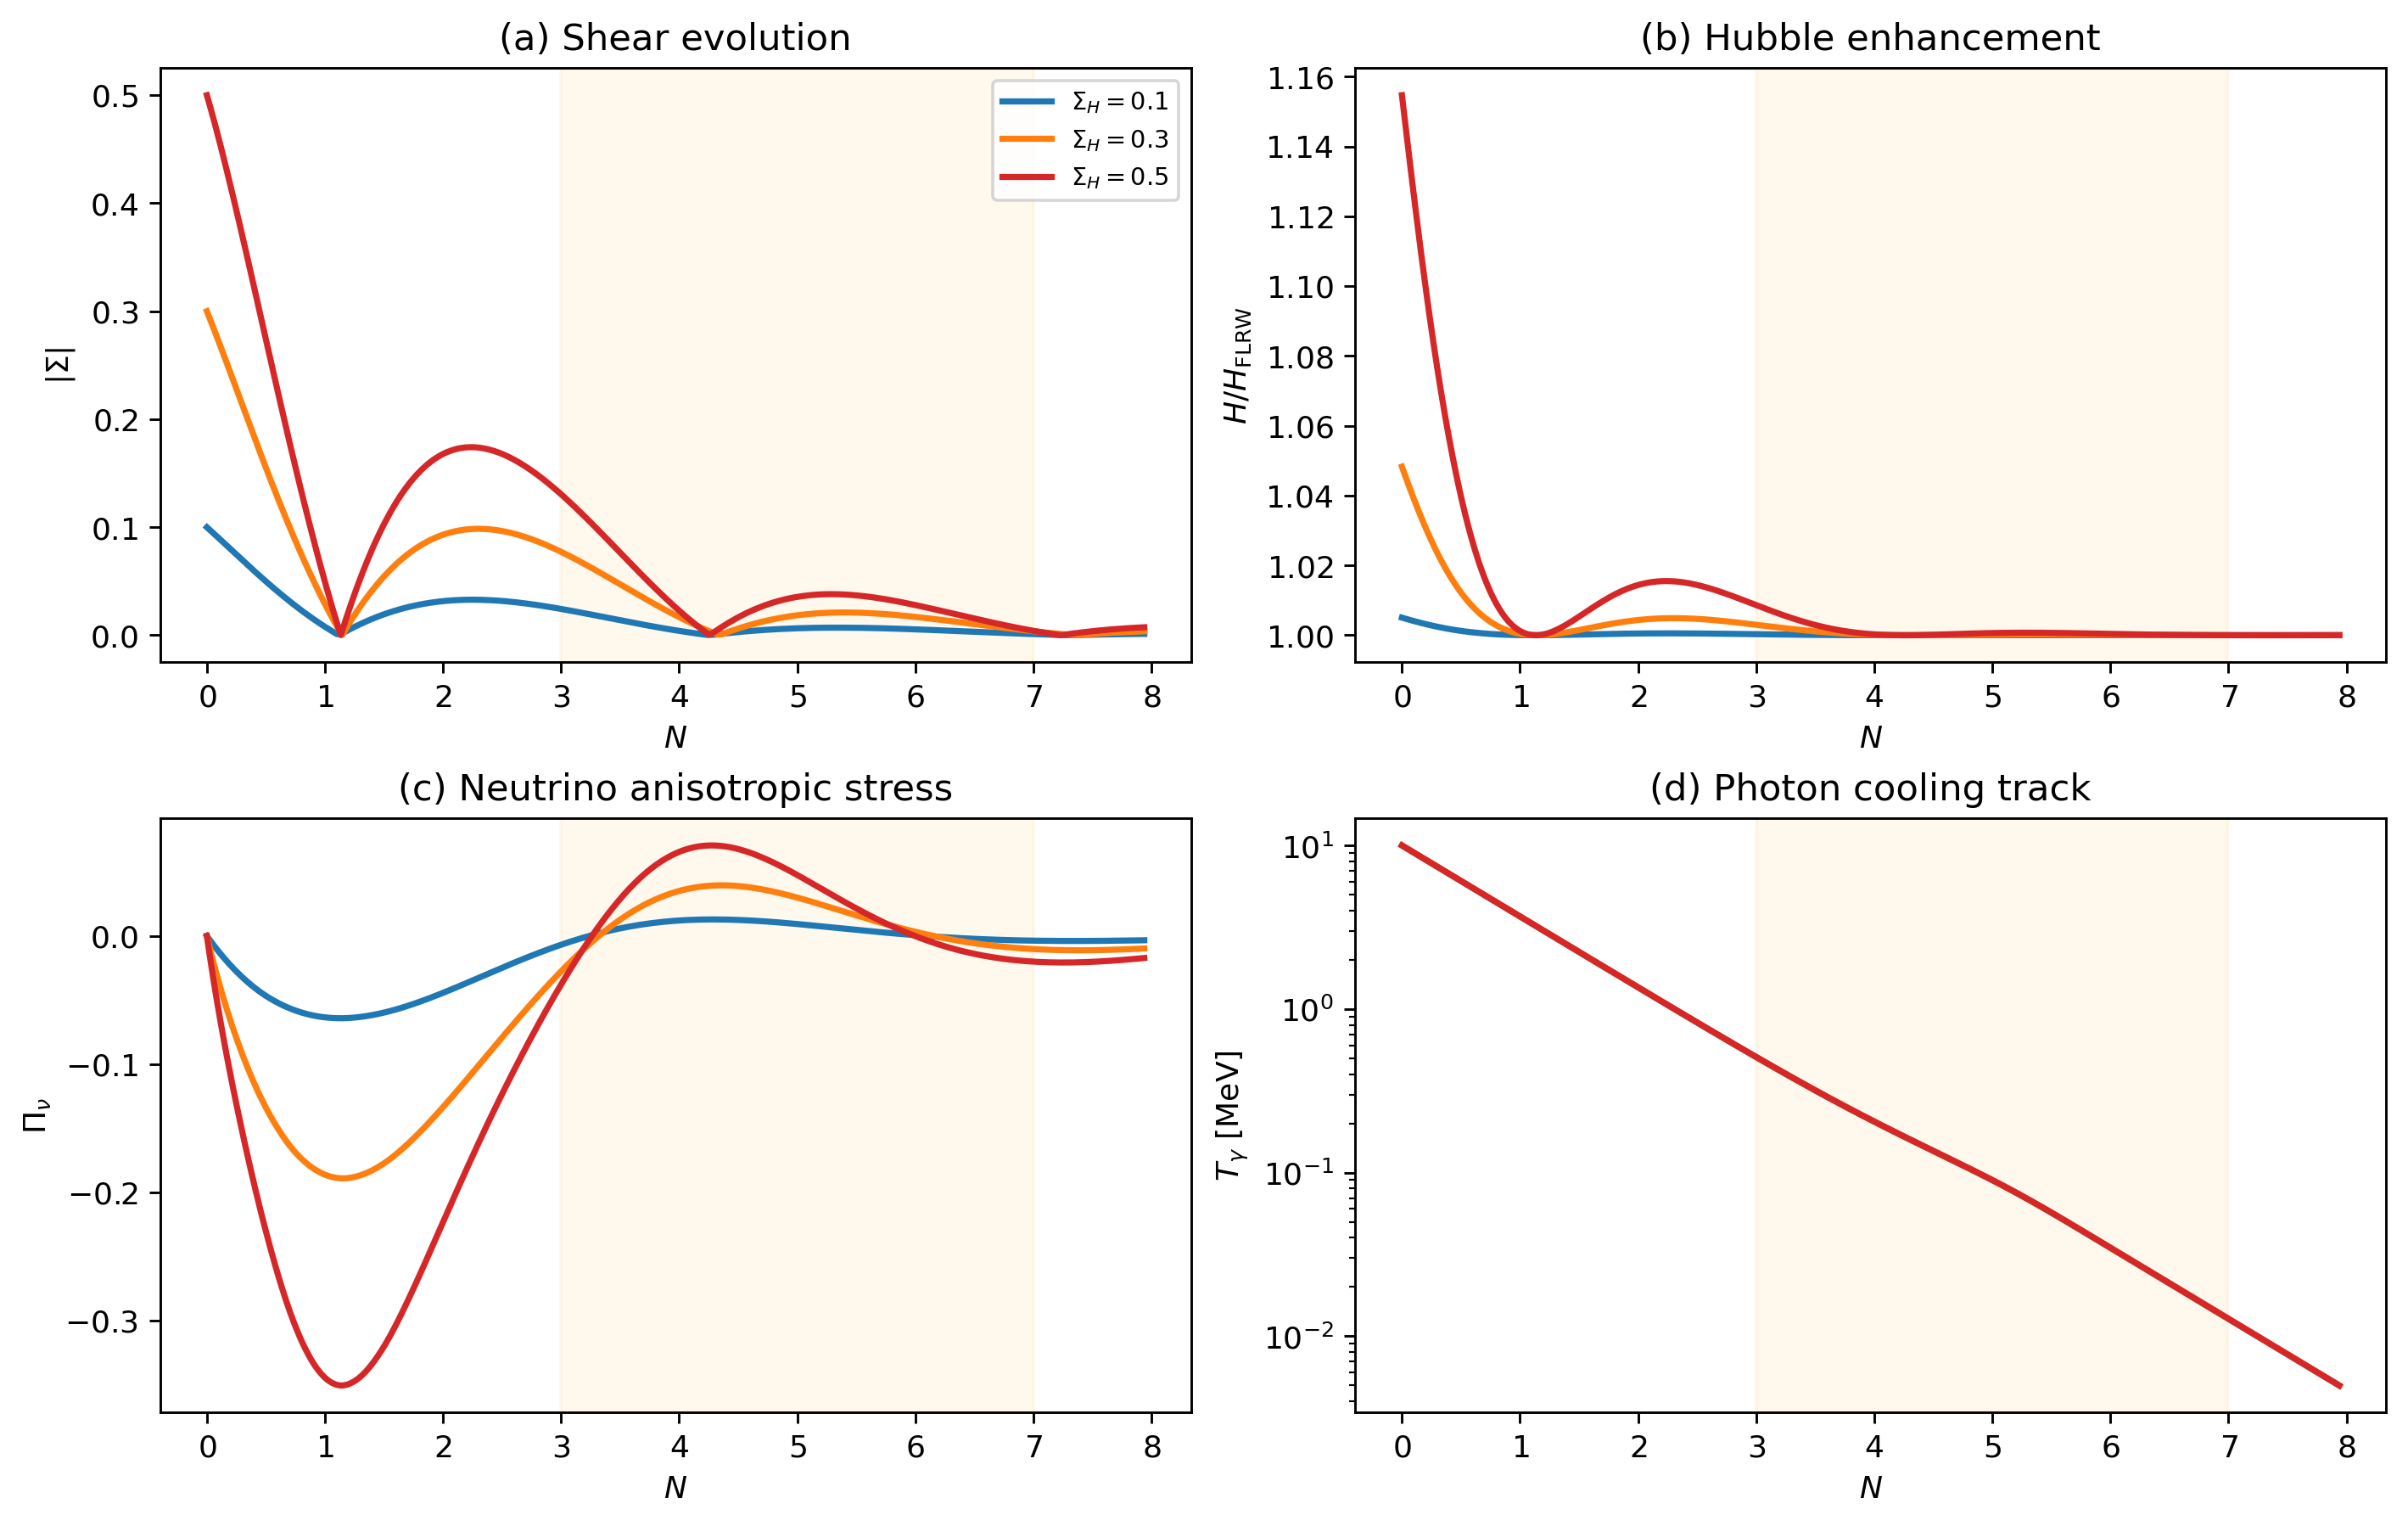
\includegraphics[width=\textwidth]{figures/fig_story_background_geometry.png}
\caption{Background geometry and cosmological evolution along the exact-characteristic reference chain.  Panels show the shear amplitude $|\Sigma|$, the Hubble enhancement $H/H_{\FLRW}$, the neutrino anisotropic stress $\Pi_\nu$, and the photon cooling track $T_\gamma(N)$ for representative initial anisotropies $\Sigma_H=0.1,0.3,0.5$.  The shaded interval marks the BBN-sensitive e-fold range.  The important point is that the geometry is not a featureless free-decay background: the characteristic neutrino sector generates a transient stress backreaction that shapes both the shear history and the expansion rate before the solution relaxes toward the FLRW attractor.}
\label{fig:story_background}
\end{figure*}

The self-consistent characteristic solution therefore differs qualitatively from the older picture in which the geometry is treated as a one-way input to the weak sector.  In the production chain the ordering is instead
\begin{equation}
(\Sigma,\Pi_\nu,H/H_{\FLRW}) \longrightarrow \tilde f_0(q) \longrightarrow (\lambda_{n\to p},\lambda_{p\to n}) \longrightarrow (\Yp,\mathrm{D/H})\,.
\end{equation}
This coupled ordering is the reason the geometry section belongs in the main production narrative rather than being relegated to a purely formal prelude.

%======================================================================
